

\documentclass[plain]{article}
\usepackage{lipsum}
\setlength{\oddsidemargin}{0.25 in}
\setlength{\evensidemargin}{-0.25 in}
\setlength{\topmargin}{-0.6 in}
\setlength{\headsep}{0.75 in}
\setlength{\parindent}{0 in}
\textwidth 6.4in
\textheight 9in
\parskip 1ex
\usepackage[framemethod=TikZ]{mdframed}
%
% ADD PACKAGES here:

 \newcommand{\argmax}{\operatornamewithlimits{argmax}}
\newcommand{\Ex}{\mathbb{E}}
\usepackage{psfrag}
\usepackage{amsmath,amsfonts,graphicx}
\usepackage{tikz}
\usepackage{mathtools}
\usepackage{bbm}
\usepackage{flexisym}
\usetikzlibrary{arrows,decorations.pathmorphing}
\newtheorem{thm}{Theorem}
\newtheorem{example}{Example}
\newtheorem{defin}{Definition}
\newtheorem{defn}{Definition}
\newtheorem{rem}{Remark}
\usepackage{framed}
\newcommand{\Pd}{\mathbb{P}}
\newtheorem{algorithm}{Algorithm}
\newtheorem{fact}{Fact}

\newcounter{lecnum}

\newcommand{\EE}{ \mathsf{E} }
\newcommand{\Var}{ \mbox{Var} }
\newcommand{\Cov}{ \mbox{Cov} }
\newcommand{\1}{\mathbbm{1}}
\newcommand{\bT}{\bar{T}}
\newcommand{\bZ}{\bar{Z}}
\newcommand{\Prob}{ \mathsf{P} }
\newcommand{\disfrac}[2]{ {\displaystyle \frac{#1}{#2}} }
\newcommand{\texfrac}[2]{ {\textstyle \frac{#1}{#2}} }
\newcommand{\dissum}[2]{ {\displaystyle \sum_{#1}^{#2}} }
\newcommand{\OR}{ \mbox{~or~} }
\newcommand{\cond}[1]{ \left|\,#1\right. }
\newcommand{\ith}[1]{ #1^{\mbox{\tiny th}} }
\newcommand{\matgen}[1]{ \left[ \begin{array}#1 \end{array} \right] }

\newcommand{\RR}{ {\bf R} }
\newcommand{\NN}{ {\bf N} }
\newcommand{\II}{ {\bf I} }
\newcommand{\ee}{ {\bf e} }
\newcommand{\LL}{ {\bf L} }
\newcommand{\PP}{ {\bf P} }
\newcommand{\calF}{ {\cal F} }
\newcommand{\One}{ \mbox{\sffamily 1} }
\newcommand{\ZZ}{ {\bf Z} }

\newcommand{\R}{{\sf R\hspace*{-0.9ex}%
\rule{0.15ex}{1.5ex}\hspace*{0.9ex}}}
\newcommand{\N}{{\sf N\hspace*{-1.0ex}%
\rule{0.15ex}{1.3ex}\hspace*{1.0ex}}}
\newcommand{\Q}{{\sf Q\hspace*{-1.1ex}%
\rule{0.15ex}{1.5ex}\hspace*{1.1ex}}}
\newcommand{\C}{{\sf C\hspace*{-0.9ex}%
\rule{0.15ex}{1.3ex}\hspace*{0.9ex}}}

\newcommand{\ds}{ \displaystyle }

%
% The following macro is used to generate the header.
%
\newcommand{\lecture}[4]{
   \pagestyle{myheadings}
   \thispagestyle{plain}
   \newpage
   \setcounter{lecnum}{#1}
   \setcounter{page}{1}
   \noindent
   \begin{center}
   \framebox{
      \vbox{\vspace{2mm}
    \hbox to 6.28in { {\bf ORIE 6360: Optimization Under Uncertainty: Robust and Online Models }
	\hfill Spring 2022} 
       \vspace{4mm}
       \hbox to 6.28in { {\Large \hfill Lecture #1 (#2)  \hfill} }
       \vspace{2mm}
       \hbox to 6.28in { {\hfill \it Professor: #3} }
      \vspace{2mm}
       \hbox to 6.28in { {\hfill \it Scribe: #4} }
      \vspace{2mm}}
   }
   \end{center}
   \markboth{Lecture #1 (#2)}{Lecture #1 (#2)}
%   {\bf Disclaimer}: {\it These notes have not been subjected to the
%   usual scrutiny reserved for formal publications.  They may be distributed
%   outside this class only with the permission of the Instructor.}
   \vspace*{4mm}
}

% Convention for citations is authors' initials followed by the year.
% For example, to cite a paper by Leighton and Maggs you would type
% \cite{LM89}, and to cite a paper by Strassen you would type \cite{S69}.
% (To avoid bibliography problems, for now we redefine the \cite command.)
% Also commands that create a suitable format for the reference list.
\renewcommand{\cite}[1]{[#1]}
% \def\beginrefs{\begin{list}%
%         {[\arabic{equation}]}{\usecounter{equation}
%          \setlength{\leftmargin}{2.0truecm}\setlength{\labelsep}{0.4truecm}%
%          \setlength{\labelwidth}{1.6truecm}}}
% \def\endrefs{\end{list}}
\def\bibentry#1{\item[\hbox{[#1]}]}

%Use this command for a figure; it puts a figure in wherever you want it.
%usage: \fig{NUMBER}{SPACE-IN-INCHES}{CAPTION}
% \newcommand{\fig}[3]{
% 			\vspace{#2}
% 			\begin{center}
% 			Figure \thelecnum.#1:~#3
% 			\end{center}
% 	}
% Use these for theorems, lemmas, proofs, etc.
%\newtheorem{theorem}{Theorem}[lecnum]
% \newtheorem{lemma}[theorem]{Lemma}
% \newtheorem{proposition}[theorem]{Proposition}
% \newtheorem{claim}[theorem]{Claim}
% \newtheorem{corollary}[theorem]{Corollary}
% \newtheorem{definition}[theorem]{Definition}
% \newenvironment{proof}{{\bf Proof:}}{\hfill\rule{2mm}{2mm}}

% **** IF YOU WANT TO DEFINE ADDITIONAL MACROS FOR YOURSELF, PUT THEM HERE:
\newcommand\E{\mathbb{E}}
\begin{document}
%FILL IN THE RIGHT INFO.
%\lecture{**LECTURE-NUMBER**}{**DATE**}{**LECTURER**}
%\solutions{**LECTURE-NUMBER**}{**DATE**}{**LECTURER**}

\lecture{23}{The Secretary Problem}{Omar El Housni}{Justin Chiu}
In this lecture we introduce the secretary problem,
a classical problem in optimal stopping.

\section{Problem Setup}
Imagine that we are an employer, interviewing candidates for a job opening.
As we have both limited resources and a tight deadline,
we can only interview at most $n$ candidates
(equivalent to drawing from a pool of $n$ candidates without replacement).
We assume the candidates are interviewed online in a \underline{random} order.

After each candidate is interviewed, we make an irrevocable decision to either
accept or reject them.
Accepting a candidate means closing the job opening and terminating our search,
while rejecting a candidate
means we can continue the search by sampling a new candidate without replacement.

\textbf{Objective:} The goal is to maximize the probability of selecting the best
candidate among the $n$ total candidates.
The main question we must answer is: When should we accept a candidate and stop searching?
Intuitively, we will break the search into two phases: explore and exploit.
In the explore phase, we will gather information on candidate quality, then use that information
in the exploit phase to make an informed selection.
This leads naturally to the idea of a threshold policy.

\textbf{Threshold policy:} In the exploration phase, we sample $x$ candidates
and reject all of them.
We use the information gathered in this phase to set an acceptance threshold
based on the maximum score of the $x$ rejected candidates.
In the subsequent exploitation phase, you accept the first candidate whose score beats
this threhshold, rejecting all others.
We illustrate this process in Figure \ref{fig:threshold-policy}.

\begin{figure}[hbt!]
\centering
\begin{tikzpicture}
% Threshold = dotted line at max in [0,x]
\draw[-] (0,.8) -- (10,.8);

% Bars for each sample
\draw[fill=red!20] (.8,0) rectangle (1.2,.4);
\draw[fill=red!20] (1.8,0) rectangle (2.2,.8);
\draw[fill=red!20] (2.8,0) rectangle (3.2,.3);
\draw[fill=red!20] (4.8,0) rectangle (5.2,.4);
\draw[fill=red!20] (5.8,0) rectangle (6.2,.6);
\draw[fill=green!20] (6.8,0) rectangle (7.2,1);

% Nodes for each sample
%\draw[thick, -] (0,-.2) -- (0,.2) node[below=1em, text height=1em] {1};
\draw[thick, -] (1,-.2) -- (1,.2) node[below=1em, text height=1em] {1};
\draw[thick, -] (2,-.2) -- (2,.2) node[below=1em, text height=1em] {2};
\draw[thick, -] (3,-.2) -- (3,.2) node[below=1em, text height=1em] {3};
\draw (4,0) node[below=0.8em, text height=1em] {$\cdots$};
\draw[thick, -] (5,-.2) -- (5,.2) node[below=1em, text height=1em] {$x$};
\draw[thick, -] (6,-.2) -- (6,.2) node[below=1em, text height=1em] {$x+1$};
\draw[thick, -] (7,-.2) -- (7,.2) node[below=1em, text height=1em] {$x+2$};
\draw[thick, -] (8,0) node[below=0.8em, text height=.8em] {$\cdots$};
\draw[thick, -] (9,-.2) -- (9,.2) node[below=1em, text height=1em] {$n$};
%\draw[ultra thick, ->] (0,0) -- (10,0) node[right,below] {$t$};
\draw[ultra thick, ->] (0,0) -- (10,0);

% Explore exploit division
\draw[thick, -] (5.5,-.8) -- (5.5,1.8);
\node (explore) at (2.75,1.5) {Phase 1: Explore};
\node (exploit) at (7.75,1.5) {Phase 2: Exploit};

\end{tikzpicture}
\vspace{-1em}
\caption{
\label{fig:threshold-policy}
The scores of each candidate are given by the height of the corresponding rectangle.
The threshold policy's exploration phase rejects the first $x$ candidates
(the rejected candidates are in red).
Following this, we choose an acceptance threshold equal to the max among the first $x$ candidates.
In this example, the acceptance threshold is determined by candidate 2.
For the exploitation phase, the first candidate that exceeds this threshold is accepted
(the accepted candidate is in green).
}
\end{figure}

The next question we must answer is how to determine the optimal explore-exploit tradeoff
by setting $x$, the number of candidates in the explore phase.
It turns out the optimal value of $x$ is approximately $n/e$.
To derive this, we will first determine the probability that the threshold policy
selects the best candidate as a function of $x$, then optimize for the best $x$.

\textbf{Derivation:}
The probability the threshold policy selects the best candidate (for a fixed $x$) is given by
\begin{align*}
\Prob(\text{select the best})
&= \sum_{j=x+1}^n \Prob(j\text{ is the best} \wedge \text{policy selects }j)\\
&= \sum_{j=x+1}^n \Prob(\text{policy selects }j\mid j\text{ is the best})
    \underbrace{\Prob(j\text{ is the best})}_{\frac{1}{n}}\\
&= \frac{1}{n}\sum_{j=x+1}^n\Prob(\text{best among }\{1,\ldots,j-1\}\text{ is in }\{1,\ldots,x\})\\
&= \frac{1}{n}\sum_{j=x+1}^n\frac{x}{j-1}\\
&= \frac{x}{n}\left(\sum_{j=1}^{n-1}\frac{1}{j} - \sum_{j=1}^{x-1}\frac{1}{j}\right)\\
&\approx \frac{x}{n} \left[ \log(n-1) - \log(x-1) \right]
\underset{n\to\infty}{\approx} \frac{x}{n}\log\frac{n}{x}.
\end{align*}
We can then maximize over $x$.
Let
\begin{align*}
f(x) &= x \log \frac{n}{x}\\
f'(x) &= \log \frac{n}{x} + x\left(-\frac{1}{x}\right)\\
&= \log n - \log x - 1 = 0\\
&\Rightarrow \log x = \log \frac{n}{e}\\
&\Rightarrow x^* = \frac{n}{e} \approx .37 n,
\end{align*}
meaning you should explore 37\% of the time
then pick the first candidate that exceeds all the scores of the first 37\% candidates.

\end{document}





